\newpage
\section{TEST 1}
% \documentclass{exam}
% % Template-specific packages
\usepackage[utf8]{inputenc} % Required for inputting international characters
\usepackage[T1]{fontenc} % Output font encoding for international characters
\usepackage{mathpazo} % Use the Palatino font

\usepackage{graphicx} % Required for including images

\usepackage{booktabs} % Required for better horizontal rules in tables

\usepackage{listings} % Required for insertion of code

\usepackage{enumerate} % To modify the enumerate environment
\usepackage{hyperref}
\usepackage{listings}
\lstset{
basicstyle=\small\ttfamily,
columns=flexible,
breaklines=true
}
\usepackage[utf8]{inputenc}
\usepackage{listings}

\lstset{
basicstyle=\small\ttfamily,
columns=flexible,
breaklines=true
}
\usepackage{fancyvrb}
\usepackage{enumitem}
\usepackage{graphicx}
\usepackage{geometry}
 \geometry{
 a4paper,
 total={6in , 10in},
 left=20mm,
 top=10mm,
 }
 
\usepackage{hyperref} 

\usepackage{graphicx}

\usepackage{listings}
\usepackage{enumitem}
\lstset{
basicstyle=\small\ttfamily,
columns=flexible,
breaklines=true
}

%\begin{document}
 
\begin{center}
\fbox{\fbox{\parbox{5.5in}{\centering
CSD2206 Section ONE Test 1   5\% of final grade:
Total 70 Marks}}}
\end{center}
 
\makebox[\textwidth]{\enspace\ }
\vspace{2cm}
\makebox[\textwidth]{Name and Student ID:\enspace\hrulefill}

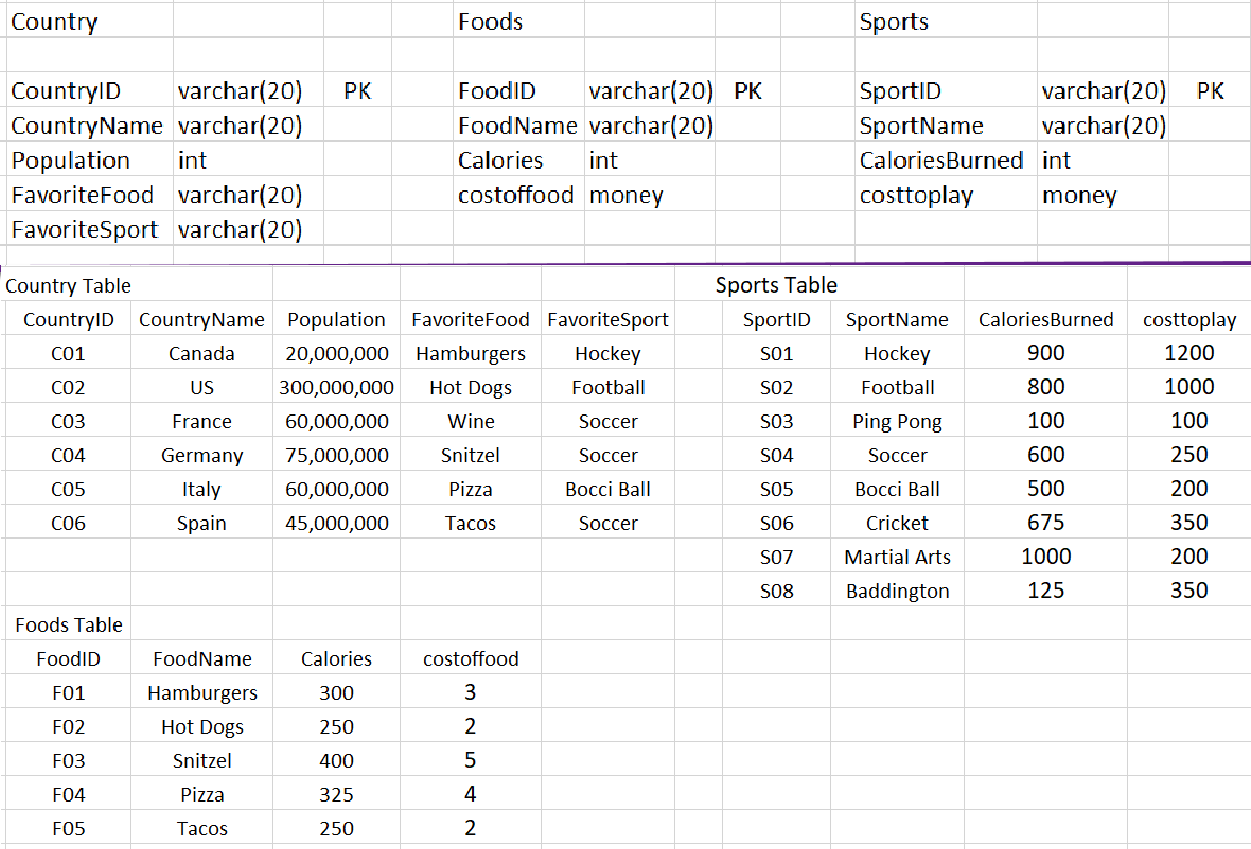
\includegraphics[scale=.5]{images/CountriesDatabaseImage.png}
\newline

\begin{questions}

\question 10 Marks: Write a SQL Statement to print out the SUM of all the 
calories BURNED by all the Sports Players in ALL COUNTRIES.
\vspace{4cm}

\question 10 Marks: Write a SQL Statement to print out the FAVORITE FOODS ORGANIZED BY FAVORITE SPORT:
\vspace{4cm}

\question 10 Marks: Write a VIEW to display much money is spent PER COUNTRY on Sports:
\vspace{4cm}

\question 10 Marks: Write a SQL Statement to create a new Country Table Record for Australia. For the values, make up some values that you think are probably correct:
\vspace{4cm}

\question 10 Marks: Write a SQL statement to print out a THE COST OF FOODS of the countries whose sports burn MORE THAN 600 calories:
\vspace{4cm}


\question 5 Marks: What is a ROWSET?
\vspace{4cm}

\question 5 Marks: What are the key features of the RELATIONAL DATABASE MODEL? When would it NOT be applicable?
\vspace{5cm}

\question 5 Marks: Why do you LOVE 1NF ?
\vspace{4cm}


\question 5 Marks: Describe Stored Procedures - What are they? Why do we use them? How do we use them?
\vspace{3cm}



\end{questions}

\end{document}
